\section{Introduction}

Science is aiming towards open and reproducible research. In gamma-ray astronomy, especially for ground-based imaging atmospheric Cherenkov telescopes (IACT), data and software have so far been mostly private to the collaboration operating the telescopes. The Cherenkov Telescope Array (CTA), the next generation of IACT, will be operated as an an open observatory, meaning that data and analysis softwares will be public at the end-user, science tools level. Momentum was thus given to the development of open data format and open-source software for gamma-ray astronomy, leading to synergies between experiments, ground based and space missions.

This is illustrated in Figure~\ref{fig:purpose}: there are many gamma-ray data producers and science tools to work with gamma-ray data, so agreeing on common data models and formats that cover most common analysis cases makes things simpler for data producers, tool developers and users.

\begin{figure}[tb]
  \centerline{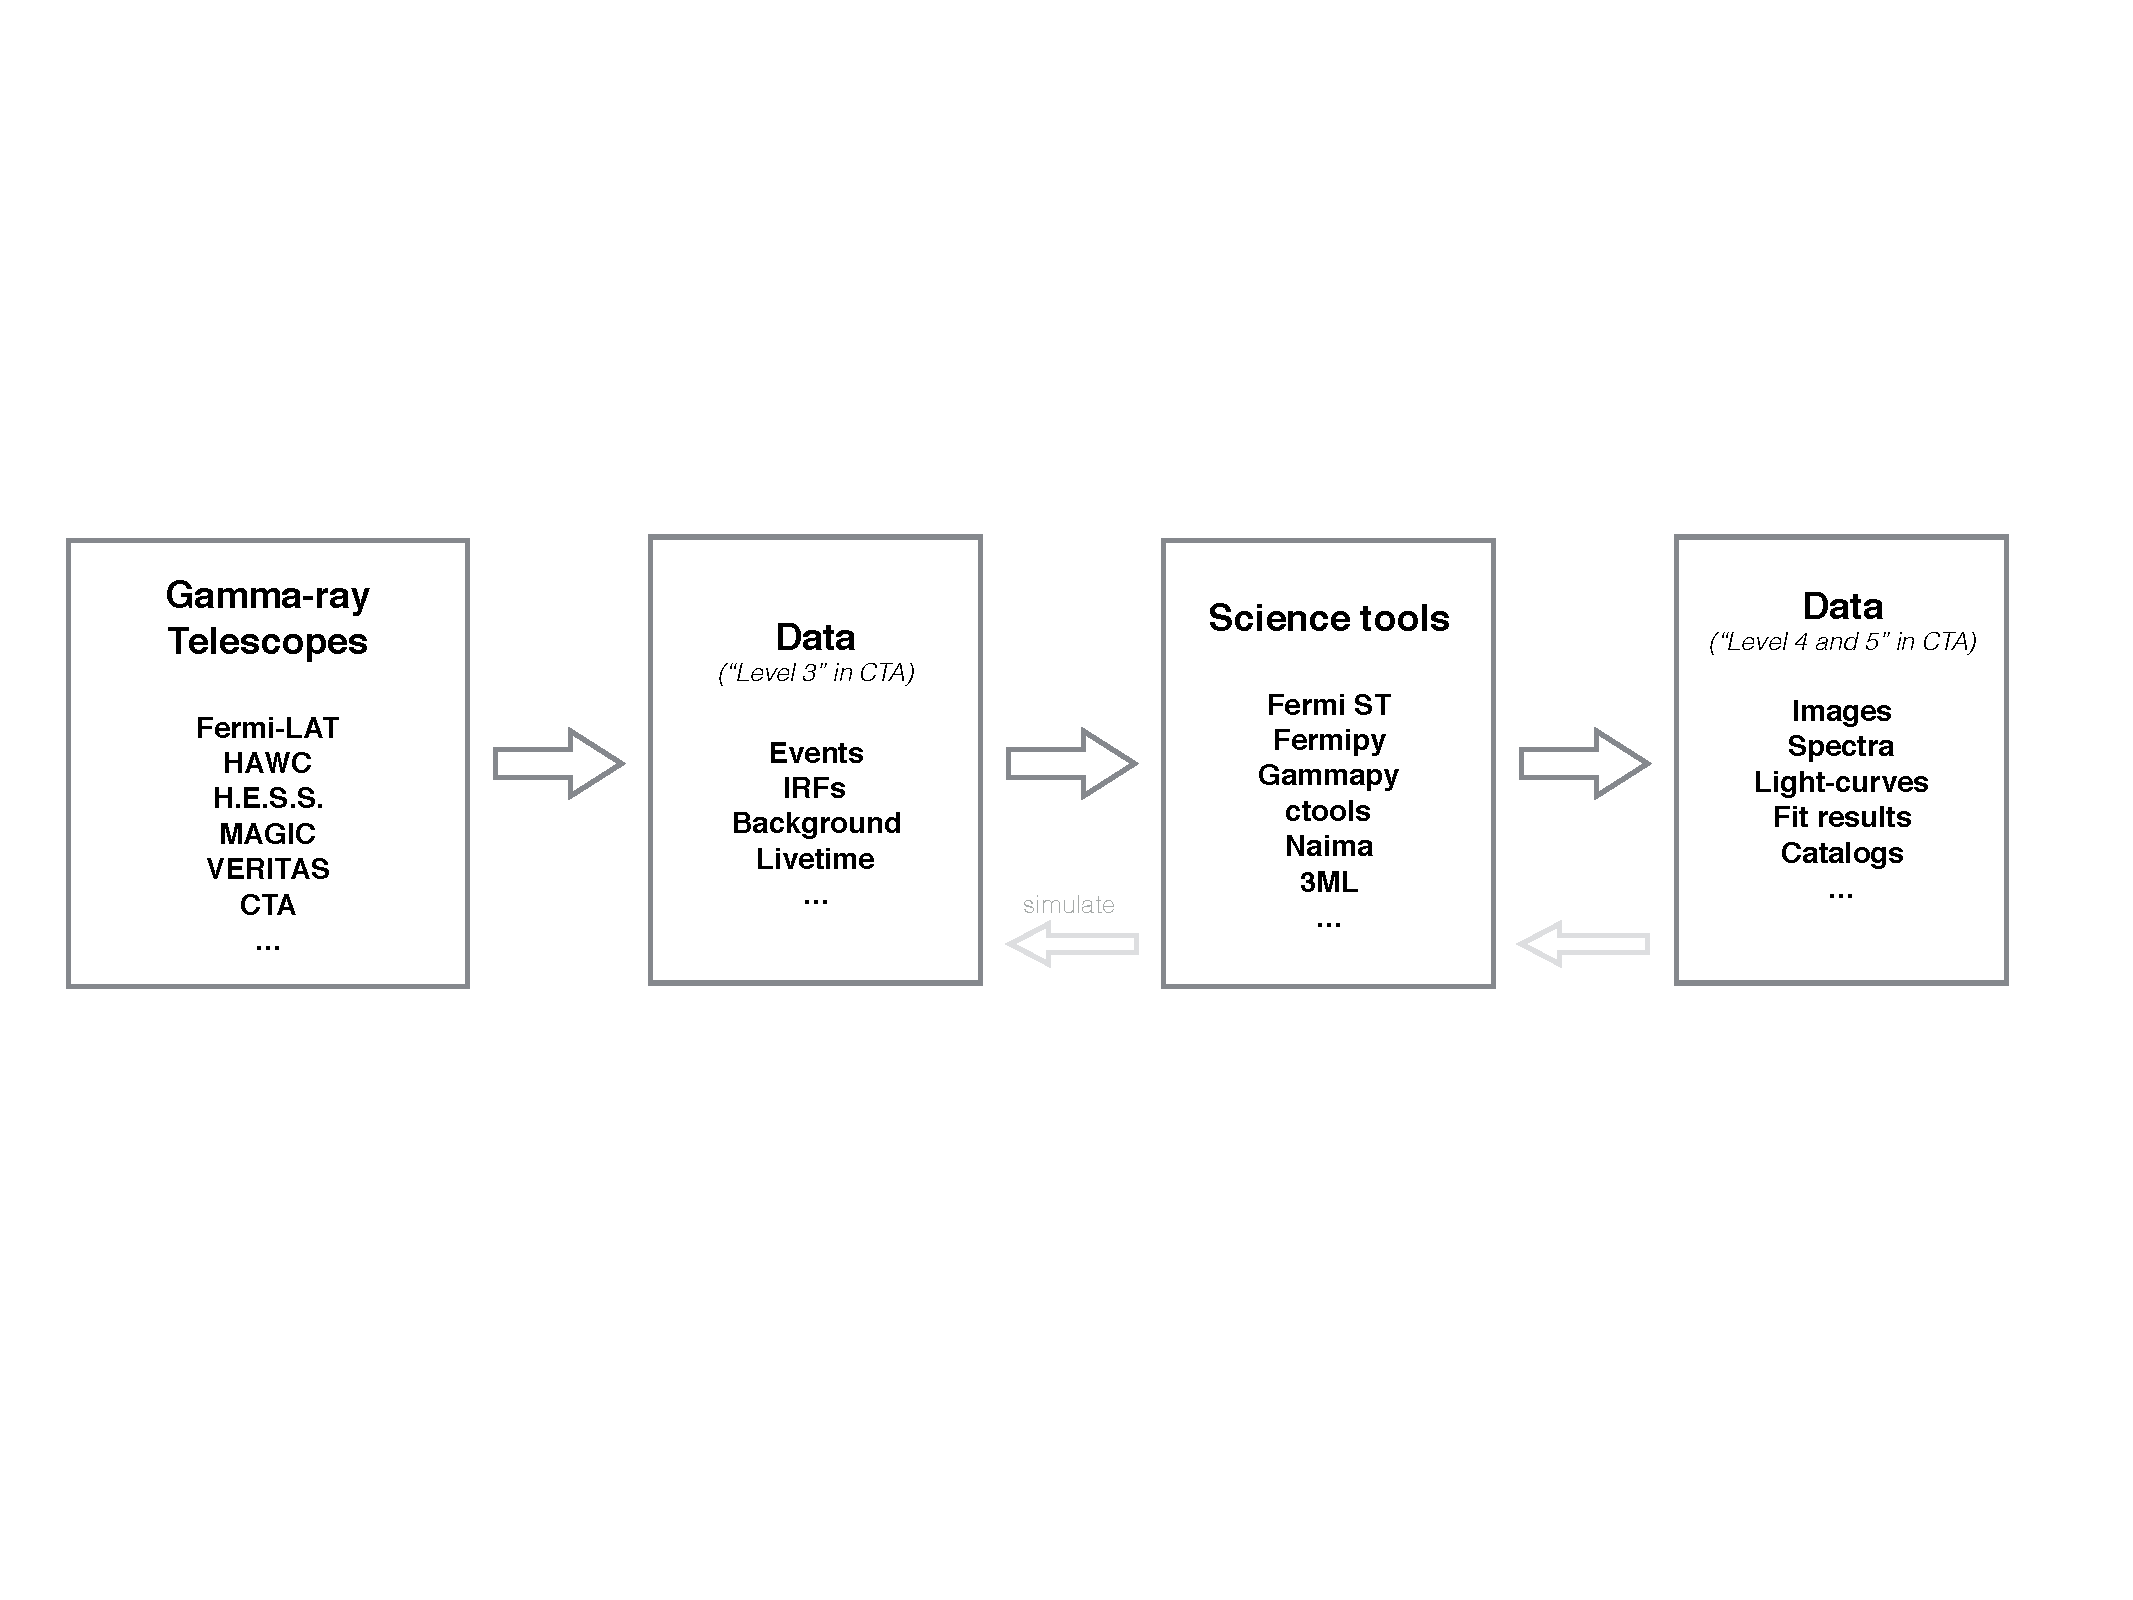
\includegraphics[width=\textwidth]{figures/purpose}}
  \caption{The purpose of the \texttt{gamma-astro-data-formats} effort: there's
  many gamma-ray data producers and consumers.}
  \label{fig:purpose}
\end{figure}

Open source analysis tools for VHE gamma-ray astronomy have emerged. They all meet on common ground of using FITS files for data transfer. The current IACTs (H.E.S.S., MAGIC and VERITAS) all use their own software based on the ROOT library, which makes it impossible to analyze the respective data with anything else than the corresponding software. Current open source analysis tools provide alternative analysis techniques compared to the present standard in VHE astronomy. It is assumed that these techniques (e.g. 3D likelihood analysis such as already implemented for Fermi-LAT) improve the sensitivity of IACTs by roughly 20\%. The data model for CTA is currently being developed but still work in progress. A main point of defining the high level data format for CTA is to understand the instrument including its systematics and IRF dependencies. In addition the needs from a user perspective have to be taken into account to create a solution as simple as possible. Having agreed on a common data format for files and on a way how to store and access those files (folder structure), makes mid-level (event energies, positions) and high-level (source position, morphology, spectrum) checks between the different chains, algorithms and open-source tools possible. This will also ease interoperability with other codes (e.g. to check results, combine results in one plot, ...). Currently two open-source science tools packages are being designed for current IACT and CTA data analysis, Gammapy (\cite{2015arXiv150907408D}) and Ctools (\cite{2016AnA...593A...1K}). Gammapy is an in-development Astropy-affiliated package. Ctools is based on the GammaLib analysis framework, which is mainly written in C++.

TODO: also mention other codes: pointlike \citep{2010PhDT.......147K},
Naima \citep{2015arXiv150903319Z}, 3ML \citep{2015arXiv150708343V},
Fermipy\footnote{\url{https://github.com/fermiPy/fermipy}}, Fermi ScienceTools.

We have created a Github organization where we are developing high-level data format specifications, in accordance with astronomy standards. 
